
%\documentclass[11pts,a4paper,amsmath,amssymb,floatfix]{article}%{report}%{book}
\documentclass[12pts,a4paper,amsmath,amssymb,floatfix]{article}%{report}%{book}
\usepackage{graphicx,wrapfig,pdfpages}% Include figure files
%\usepackage{dcolumn,enumerate}% Align table columns on decimal point
\usepackage{enumerate,enumitem}% Align table columns on decimal point
\usepackage{bm,dpfloat}% bold math
\usepackage[pdftex,bookmarks,colorlinks=true,urlcolor=rltblue,citecolor=blue]{hyperref}
\usepackage{amsfonts,amsmath,amssymb,stmaryrd,indentfirst}
\usepackage{times,psfrag}
\usepackage{natbib}
\usepackage{color}
\usepackage{units}
\usepackage{rotating}
\usepackage{multirow}


\usepackage{pifont}
\usepackage{subfigure}
\usepackage{subeqnarray}
\usepackage{ifthen}

\usepackage{supertabular}
\usepackage{moreverb}
\usepackage{listings}
\usepackage{palatino}
%\usepackage{doi}
\usepackage{longtable}
\usepackage{float}
\usepackage{perpage}
\MakeSorted{figure}
%\usepackage{pdflscape}


%\usepackage{booktabs}
%\newcommand{\ra}[1]{\renewcommand{\arraystretch}{#1}}


\definecolor{rltblue}{rgb}{0,0,0.75}


%\usepackage{natbib}
\usepackage{fancyhdr} %%%%
\pagestyle{fancy}%%%%
% with this we ensure that the chapter and section
% headings are in lowercase
%%%%\renewcommand{\chaptermark}[1]{\markboth{#1}{}}
\renewcommand{\sectionmark}[1]{\markright{\thesection\ #1}}
\fancyhf{} %delete the current section for header and footer
\fancyhead[LE,RO]{\bfseries\thepage}
\fancyhead[LO]{\bfseries\rightmark}
\fancyhead[RE]{\bfseries\leftmark}
\renewcommand{\headrulewidth}{0.5pt}
% make space for the rule
\fancypagestyle{plain}{%
\fancyhead{} %get rid of the headers on plain pages
\renewcommand{\headrulewidth}{0pt} % and the line
}

\def\newblock{\hskip .11em plus .33em minus .07em}
\usepackage{color}

%\usepackage{makeidx}
%\makeindex

\setlength\textwidth      {16.cm}
\setlength\textheight     {22.6cm}
\setlength\oddsidemargin  {-0.3cm}
\setlength\evensidemargin {0.3cm}

\setlength\headheight{14.49998pt} 
\setlength\topmargin{0.0cm}
\setlength\headsep{1.cm}
\setlength\footskip{1.cm}
\setlength\parskip{0pt}
\setlength\parindent{0pt}


%%%
%%% Headers and Footers
\lhead[] {\text{\small{EG3029 -- Chemical Thermodynamics}}} 
\rhead[] {{\text{\small{Lab Exercise 2: UniSim (2014/15)}}}}
%\chead[] {\text{\small{Session 2012/13}}} 
\lfoot[]{Dr Jeff Gomes}
%\cfoot[\thepage]{\thepage}
\rfoot[\text{\small{\thepage}}]{\thepage}
\renewcommand{\headrulewidth}{0.8pt}


%%%
%%% space between lines
%%%
\renewcommand{\baselinestretch}{1.5}

\newenvironment{VarDescription}[1]%
  {\begin{list}{}{\renewcommand{\makelabel}[1]{\textbf{##1:}\hfil}%
    \settowidth{\labelwidth}{\textbf{#1:}}%
    \setlength{\leftmargin}{\labelwidth}\addtolength{\leftmargin}{\labelsep}}}%
  {\end{list}}

%%%%%%%%%%%%%%%%%%%%%%%%%%%%%%%%%%%%%%%%%%%
%%%%%%                              %%%%%%%
%%%%%%      NOTATION SECTION        %%%%%%%
%%%%%%                              %%%%%%%
%%%%%%%%%%%%%%%%%%%%%%%%%%%%%%%%%%%%%%%%%%%

% Text abbreviations.
\newcommand{\ie}{{\em{i.e., }}}
\newcommand{\eg}{{\em{e.g., }}}
\newcommand{\cf}{{\em{cf., }}}
\newcommand{\wrt}{with respect to}
\newcommand{\lhs}{left hand side}
\newcommand{\rhs}{right hand side}
% Commands definining mathematical notation.

% This is for quantities which are physically vectors.
\renewcommand{\vec}[1]{{\mbox{\boldmath$#1$}}}
% Physical rank 2 tensors
\newcommand{\tensor}[1]{\overline{\overline{#1}}}
% This is for vectors formed of the value of a quantity at each node.
\newcommand{\dvec}[1]{\underline{#1}}
% This is for matrices in the discrete system.
\newcommand{\mat}[1]{\mathrm{#1}}


\DeclareMathOperator{\sgn}{sgn}
\newtheorem{thm}{Theorem}[section]
\newtheorem{lemma}[thm]{Lemma}

%\newcommand\qed{\hfill\mbox{$\Box$}}
\newcommand{\re}{{\mathrm{I}\hspace{-0.2em}\mathrm{R}}}
\newcommand{\inner}[2]{\langle#1,#2\rangle}
\renewcommand\leq{\leqslant}
\renewcommand\geq{\geqslant}
\renewcommand\le{\leqslant}
\renewcommand\ge{\geqslant}
\renewcommand\epsilon{\varepsilon}
\newcommand\eps{\varepsilon}
\renewcommand\phi{\varphi}
\newcommand{\bmF}{\vec{F}}
\newcommand{\bmphi}{\vec{\phi}}
\newcommand{\bmn}{\vec{n}}
\newcommand{\bmns}{{\textrm{\scriptsize{\boldmath $n$}}}}
\newcommand{\bmi}{\vec{i}}
\newcommand{\bmj}{\vec{j}}
\newcommand{\bmk}{\vec{k}}
\newcommand{\bmx}{\vec{x}}
\newcommand{\bmu}{\vec{u}}
\newcommand{\bmv}{\vec{v}}
\newcommand{\bmr}{\vec{r}}
\newcommand{\bma}{\vec{a}}
\newcommand{\bmg}{\vec{g}}
\newcommand{\bmU}{\vec{U}}
\newcommand{\bmI}{\vec{I}}
\newcommand{\bmq}{\vec{q}}
\newcommand{\bmT}{\vec{T}}
\newcommand{\bmM}{\vec{M}}
\newcommand{\bmtau}{\vec{\tau}}
\newcommand{\bmOmega}{\vec{\Omega}}
\newcommand{\pp}{\partial}
\newcommand{\kaptens}{\tensor{\kappa}}
\newcommand{\tautens}{\tensor{\tau}}
\newcommand{\sigtens}{\tensor{\sigma}}
\newcommand{\etens}{\tensor{\dot\epsilon}}
\newcommand{\ktens}{\tensor{k}}
\newcommand{\half}{{\textstyle \frac{1}{2}}}
\newcommand{\tote}{E}
\newcommand{\inte}{e}
\newcommand{\strt}{\dot\epsilon}
\newcommand{\modu}{|\bmu|}
% Derivatives
\renewcommand{\d}{\mathrm{d}}
\newcommand{\D}{\mathrm{D}}
\newcommand{\ddx}[2][x]{\frac{\d#2}{\d#1}}
\newcommand{\ddxx}[2][x]{\frac{\d^2#2}{\d#1^2}}
\newcommand{\ddt}[2][t]{\frac{\d#2}{\d#1}}
\newcommand{\ddtt}[2][t]{\frac{\d^2#2}{\d#1^2}}
\newcommand{\ppx}[2][x]{\frac{\partial#2}{\partial#1}}
\newcommand{\ppxx}[2][x]{\frac{\partial^2#2}{\partial#1^2}}
\newcommand{\ppt}[2][t]{\frac{\partial#2}{\partial#1}}
\newcommand{\pptt}[2][t]{\frac{\partial^2#2}{\partial#1^2}}
\newcommand{\DDx}[2][x]{\frac{\D#2}{\D#1}}
\newcommand{\DDxx}[2][x]{\frac{\D^2#2}{\D#1^2}}
\newcommand{\DDt}[2][t]{\frac{\D#2}{\D#1}}
\newcommand{\DDtt}[2][t]{\frac{\D^2#2}{\D#1^2}}
% Norms
\newcommand{\Ltwo}{\ensuremath{L_2} }
% Basis functions
\newcommand{\Qone}{\ensuremath{Q_1} }
\newcommand{\Qtwo}{\ensuremath{Q_2} }
\newcommand{\Qthree}{\ensuremath{Q_3} }
\newcommand{\QN}{\ensuremath{Q_N} }
\newcommand{\Pzero}{\ensuremath{P_0} }
\newcommand{\Pone}{\ensuremath{P_1} }
\newcommand{\Ptwo}{\ensuremath{P_2} }
\newcommand{\Pthree}{\ensuremath{P_3} }
\newcommand{\PN}{\ensuremath{P_N} }
\newcommand{\Poo}{\ensuremath{P_1P_1} }
\newcommand{\PoDGPt}{\ensuremath{P_{-1}P_2} }

\newcommand{\metric}{\tensor{M}}
\newcommand{\configureflag}[1]{\texttt{#1}}

% Units
\newcommand{\m}[1][]{\unit[#1]{m}}
\newcommand{\km}[1][]{\unit[#1]{km}}
\newcommand{\s}[1][]{\unit[#1]{s}}
\newcommand{\invs}[1][]{\unit[#1]{s}\ensuremath{^{-1}}}
\newcommand{\ms}[1][]{\unit[#1]{m\ensuremath{\,}s\ensuremath{^{-1}}}}
\newcommand{\mss}[1][]{\unit[#1]{m\ensuremath{\,}s\ensuremath{^{-2}}}}
\newcommand{\K}[1][]{\unit[#1]{K}}
\newcommand{\PSU}[1][]{\unit[#1]{PSU}}
\newcommand{\Pa}[1][]{\unit[#1]{Pa}}
\newcommand{\kg}[1][]{\unit[#1]{kg}}
\newcommand{\rads}[1][]{\unit[#1]{rad\ensuremath{\,}s\ensuremath{^{-1}}}}
\newcommand{\kgmm}[1][]{\unit[#1]{kg\ensuremath{\,}m\ensuremath{^{-2}}}}
\newcommand{\kgmmm}[1][]{\unit[#1]{kg\ensuremath{\,}m\ensuremath{^{-3}}}}
\newcommand{\Nmm}[1][]{\unit[#1]{N\ensuremath{\,}m\ensuremath{^{-2}}}}

% Dimensionless numbers
\newcommand{\dimensionless}[1]{\mathrm{#1}}
\renewcommand{\Re}{\dimensionless{Re}}
\newcommand{\Ro}{\dimensionless{Ro}}
\newcommand{\Fr}{\dimensionless{Fr}}
\newcommand{\Bu}{\dimensionless{Bu}}
\newcommand{\Ri}{\dimensionless{Ri}}
\renewcommand{\Pr}{\dimensionless{Pr}}
\newcommand{\Pe}{\dimensionless{Pe}}
\newcommand{\Ek}{\dimensionless{Ek}}
\newcommand{\Gr}{\dimensionless{Gr}}
\newcommand{\Ra}{\dimensionless{Ra}}
\newcommand{\Sh}{\dimensionless{Sh}}
\newcommand{\Sc}{\dimensionless{Sc}}


% Journals
\newcommand{\IJHMT}{{\it International Journal of Heat and Mass Transfer}}
\newcommand{\NED}{{\it Nuclear Engineering and Design}}
\newcommand{\ICHMT}{{\it International Communications in Heat and Mass Transfer}}
\newcommand{\NET}{{\it Nuclear Engineering and Technology}}
\newcommand{\HT}{{\it Heat Transfer}}   
\newcommand{\IJHT}{{\it International Journal for Heat Transfer}}

\newcommand{\frc}{\displaystyle\frac}

\newlist{ExList}{enumerate}{1}
\setlist[ExList,1]{label={\bf Example 1.} {\bf \arabic*}}

\newlist{ProbList}{enumerate}{1}
\setlist[ProbList,1]{label={\bf Problem 1.} {\bf \arabic*}}

%%%%%%%%%%%%%%%%%%%%%%%%%%%%%%%%%%%%%%%%%%%
%%%%%%                              %%%%%%%
%%%%%% END OF THE NOTATION SECTION  %%%%%%%
%%%%%%                              %%%%%%%
%%%%%%%%%%%%%%%%%%%%%%%%%%%%%%%%%%%%%%%%%%%


% Cause numbering of subsubsections. 
%\setcounter{secnumdepth}{8}
%\setcounter{tocdepth}{8}

\setcounter{secnumdepth}{4}%
\setcounter{tocdepth}{4}%


\begin{document}

\begin{enumerate}[label=\bfseries Problem \arabic*]
%
\item\label{ExcessVolume} {\it (Excess Properties)} Many substances do not exhibit ideal behaviour when they are mixed with each other. One prominent example is water in mixtures with other polar chemicals including methanol and ethanol. Such non-ideal effects result from strong intermolecular interactions and often manifest in significant deviations of the mixture properties from the ideal values. Needless to say, that knowing these deviations is of great importance for designing processes in many respects. Fortunately, property deviations can be determined both numerically and experimentally in the form of excess properties. 

{\bf \textcolor{blue}{Task 1:}} Start {\bf UniSim} and open a new case. Add water and dimethyl sulphoxide (DMSO) as components. {\bf Develop a strategy} for determining the excess volume of binary water/DMSO mixtures. Using your approach determine the excess volumes of both systems with water mole fractions of 0.0, 0.1, 0.2, 0.3, 0.4, 0.5, 0.6, 0.7, 0.8, 0.9 and 1.0 with the following fluid packages:
\begin{itemize}
\item Lee-Kesler-Plocker
\item Peng-Robinson
\item Soave-Redlich-Kwong
\item NRTL
\item UNIQUAC
\end{itemize}

\clearpage
\item\label{MassBalance} {\it (Mass and Energy balances)} Here we will optimize a sugar production plant where 22680 kg.h$^{-1}$ of a 10 wt$\%$ aqueous sugar (d-glucose or Dextrose) solution at 26.7$^{\circ}$C and atmospheric pressure needs to be concentrated to 50 wt$\%$ using an evaporation process.  Dry, saturated steam is available at 202.5 kPa. The procedure to create the {\it Process Flow Diagram} (PFD) for this test-case is described below:
%
\begin{enumerate}
%
\item Open a new case in {\it UniSim}, add {\bf water} and {\bf sugar} (d-glucose or Dextrose) to your {\bf Component List} and select {\bf NRTL} as your {\bf Fluid Package}.  Enter the {\bf Simulation Environment}.
%
\item We will work through setting up a Single-Effect Evaporator operating at atmospheric pressure which will perform the concentration (Evaporation) process.  An evaporator is essentially a partially filled vessel into which we feed a dilute liquid.  At steady-state, we assume that the vessel is well mixed and that the liquid in the vessel has the same composition as the product.  The evaporation is driven by a bank of submerged tubes within which we condense steam.  We thus have condensation on the inside of the tubes and boiling on the outside of the tubes.  For the system to operate we must ensure that the saturation temperature of the steam is greater than the boiling point of the liquid.
%
\item {\it UniSim} does not have a dedicated $\lq$Evaporator' icon so our first task is to use the icons which are available to create an evaporator.  To your {\bf PFD} add a {\bf Separator} from the {\bf Palette}; this will be our evaporator vessel.  Using the {\bf Attach Mode}, create streams {\bf 1} (Feed Stream), {\bf 2} (Vapour Product) and {\bf 3} (Liquid Product).  The feed stream is our dilute sugar solution:  22680 kg.h$^{-1}$, 26.7$^{\circ}$C, 101325 kPa, 0.1 wt$\%$ d-glucose, 0.9 wt$\%$ water).
%
\item We must now tell {\it UniSim} that we would like to condense saturated steam at 202.5 kPa and deliver the latent heat to the evaporator.  From the {\bf Palette}, add a {\bf Cooler} to the sheet below and to the left of the vessel.  Using the {\bf Attach Mode}, create streams {\bf 4} (Feed) and {\bf 5} (Product).  Attach the energy stream from the Cooler to the energy stream port of the separator icon.
%
      \begin{figure}[h]
        \begin{center}
          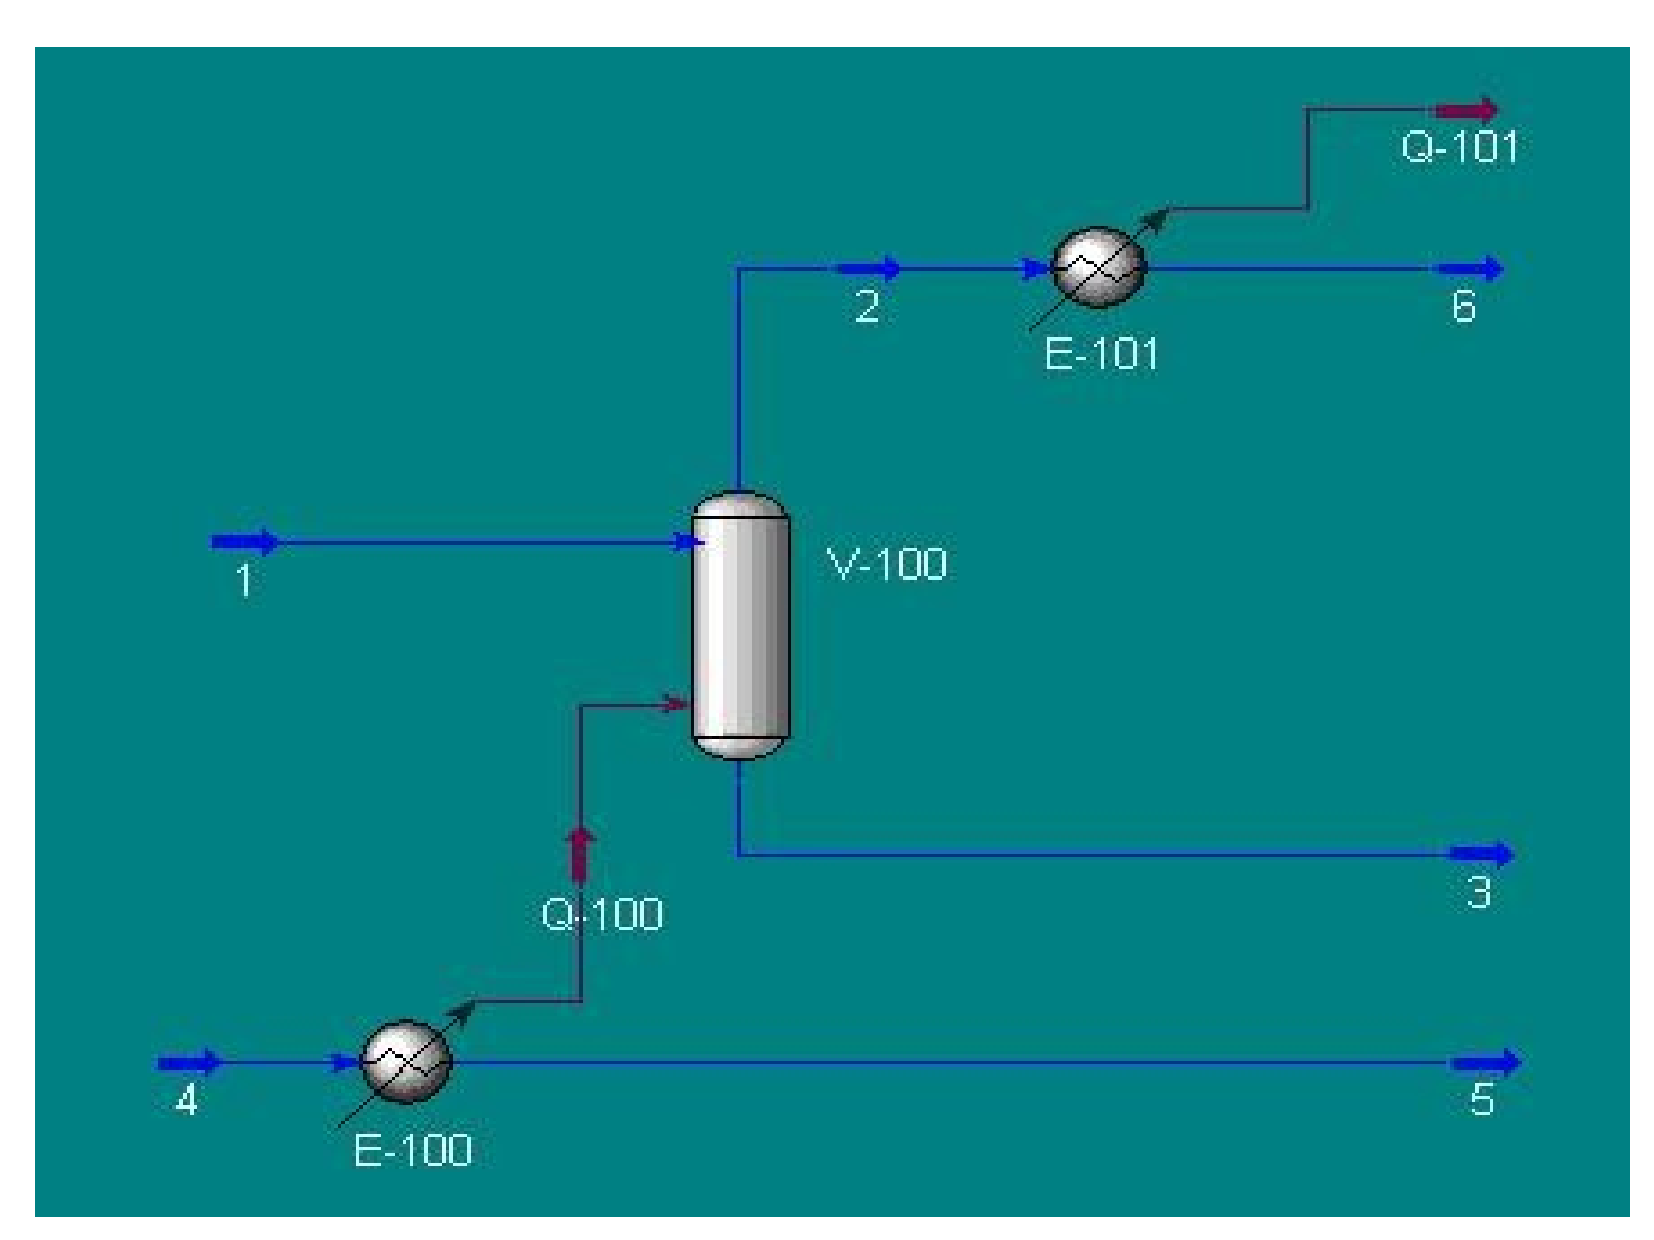
\includegraphics[width=12cm,height=8cm,clip]{./Pics/Practical2_UniSimSugar}
        \end{center}
        \caption{Snapshot of the dextrose solution evaporation PFD.}\label{sugarpic}
      \end{figure}
%
\item \textcolor{red}{{\bf Important Note:} The {\bf Vapour / Phase Fraction} field in the {\bf Conditions} window of the {\bf Worksheet Tab} allows us to specify whether a stream is saturated liquid (0), saturated vapour (1) or two-phase 0 $< x^{(v)} <$ 1.  For a pure fluid (e.g. water) the Gibbs Phase Rule tells us that we may only specify two of the variables Temperature, Pressure, Vapour Fraction.}
%
\item Specify stream {\bf 4} as having a vapour fraction of {\bf 1} (Saturated Vapour), a pressure of 202.5 kPa, a mass fraction water of 1 and a flowrate of 555.5 kgmol.h$^{-1}$.
%
\item We will assume that the condensation occurs at constant pressure (no pressure drop; idealized situation).  In the {\bf Parameters} window for the {\bf Cooler}, input 0 in the Delta P field.  {\it UniSim} now knows the flowrate, composition and pressure of the condensate stream (Stream {\bf 5}) but does not know the temperature (it may be saturated liquid or sub-cooled liquid).  Input a vapour fraction of 0 in the Vapour / Phase Fraction (saturated liquid) field for Stream {\bf 5}.
%
\item The PFD should now have computed and you should have a liquid product (Stream {\bf 3}) of 1.538$\times$10$^{4}$ kg.h$^{-1}$ containing 25.75 wt$\%$ of d-glucose.  Your heat stream from the cooler to the separator should be 6114 kW and you should be generating 7302 kg.h$^{-1}$ of superheated steam at 101.325 kPa and 108.6$^{\circ}$C.
%
\item The last stage in the completion of our single effect evaporator is to condense the steam which we have generated.  Insert a cooler which accepts your superheated steam and condenses it at constant pressure (zero pressure drop) to yield saturated liquid (Vapour / Phase Fraction = 0).
%
\item Your PFD should look like Fig.~\ref{sugarpic}.
%
\end{enumerate}
Chemical Engineers are frequently required to analyze the effect of changing one process variable on another process variable.  We will use our Evaporator to analyze the effect of changing the Feed Steam flowrate on the product composition.  More specifically, we will tell {\it UniSim} to test values of the flowrate of stream {\bf 4} from  10000 to 24000 kg.h$^{-1}$ in steps of 1000 kg.h$^{-1}$ and report the values of mass fraction d-glucose in the product (stream {\bf 3}). You may follow the steps below:
\begin{itemize}
%
\item From the {\bf Tools} menu, select the {\bf Databook}.  
\item In the {\bf Variables} tab, click on {\bf Insert}.
\item In the object list, highlight {\bf Stream 4} the in the variable list highlight {\bf Mass Flow}; click {\bf Add}.  
\item Now highlight {\bf Stream 3} in the object list and, in the variables list highlight {\bf Comp Mass Frac} (Component Mass Fraction).  In the variable specifics list highlight {\bf dextrose}.  Click on {\bf Add} then click {\bf Close}.
\item In the {\bf Databook} select the {\bf Case Studies} tab.  In the Available {\bf Case Studies} area,  click {\bf Add}.
\item {\it UniSim} will create {\bf Case Study 1}.  
\item In the {\bf Case Studies Data Selection Area} we will tell {\it UniSim} that we want to vary the mass flow rate of stream {\bf 4} and monitor its effect on the mass fraction of dextrose in stream {\bf 3}.  
\item Check the tick-box for Stream {\bf 4} in the {\bf Ind} (Independent Variable) list and check the tick-box for Stream {\bf 3} in the {\bf Dep} (Dependent Variable) list.  
\item In the {\bf Available Case Studies} area, click on {\bf View}.
\item Enter 10000 in the {\bf Low Bound} field 24000 in the {\bf High Bound} field and 1000 in the {\bf Step-Size} field. {\it UniSim} should now tell you that you are checking 15 states.  
\item Click {\bf Start} to undertake the analysis.  
\item Click {\bf Results} to view the results and;
\item You may view your results as plot, table or transposed table.
\end{itemize}

{\bf \textcolor{blue}{Task 2:}} Modify the lower bound, upper bound and step size fields to allow you to estimate the steam flow rate is required to meet the specification of 50 wt$\%$ dextrose.
%
\end{enumerate}
\clearpage

{\bf {\large Deliverables:}}
\begin{enumerate}
%
\item Write a report containing:
\begin{enumerate}
\item A brief summary of the equations of state used in both sets of simulations;
\item For \ref{ExcessVolume}: 
\begin{enumerate}
\item brief summary of excess thermodynamic properties;
\item Results (i.e., plots of excess volume $\times$ molar fraction of water for all EOS) and discussion;
\end{enumerate}
\item For \ref{MassBalance}: 
\begin{enumerate}
\item Plot of mass flow rate of superheated steam in stream {\bf 4} $\times$ molar fraction of dextrose in stream {\bf 3};
\item\label{optimal} Obtain the {\it optimal flow rate of superheated steam} (stream {\bf 4}) $\left(\text{in kg.h}^{-1}\right)$ to produce dextrose (stream {\bf 3}) at 50 wt$\%$;
\item For the {\it optimal superheated steam stream} obtained above, calculate the power extracted (in kW) in the {\bf Coolers} (E-100 and E-101) using saturated water-steam and superheated steam tables and the mass flow rate of your simulation. Compare these calculated power streams with those obtained from your optimal simulation. 
\end{enumerate}
\end{enumerate}
%
\item Prepare the report as {\bf PDF} file and submit it through Turnitin.  
%
\item The filename of the report should be {\bf EG3029$\_$UniSim$\_$Lab2$\_$XXX.pdf} ({\bf XXX} to be replaced by your surname). 
%
\item Submit your work by {\bf Sunday, November 9th 2014, 23:59} at the latest. 
%
\item Penalties for late or non-submission are as follows: for late submission, 1 CGS mark will be deducted for each day late (including weekends); submission later than 7 days after the deadline will be considered as non-submission and a CGS mark of 0 will be awarded. 
%
\item Remember to include in your electronic submission a completed plagiarism cover sheet. 
%
\item Note that the submitted work is part of the continuous assessment which will contribute 20$\%$ to your EG3029 mark.
%
\end{enumerate}



\clearpage

%{
%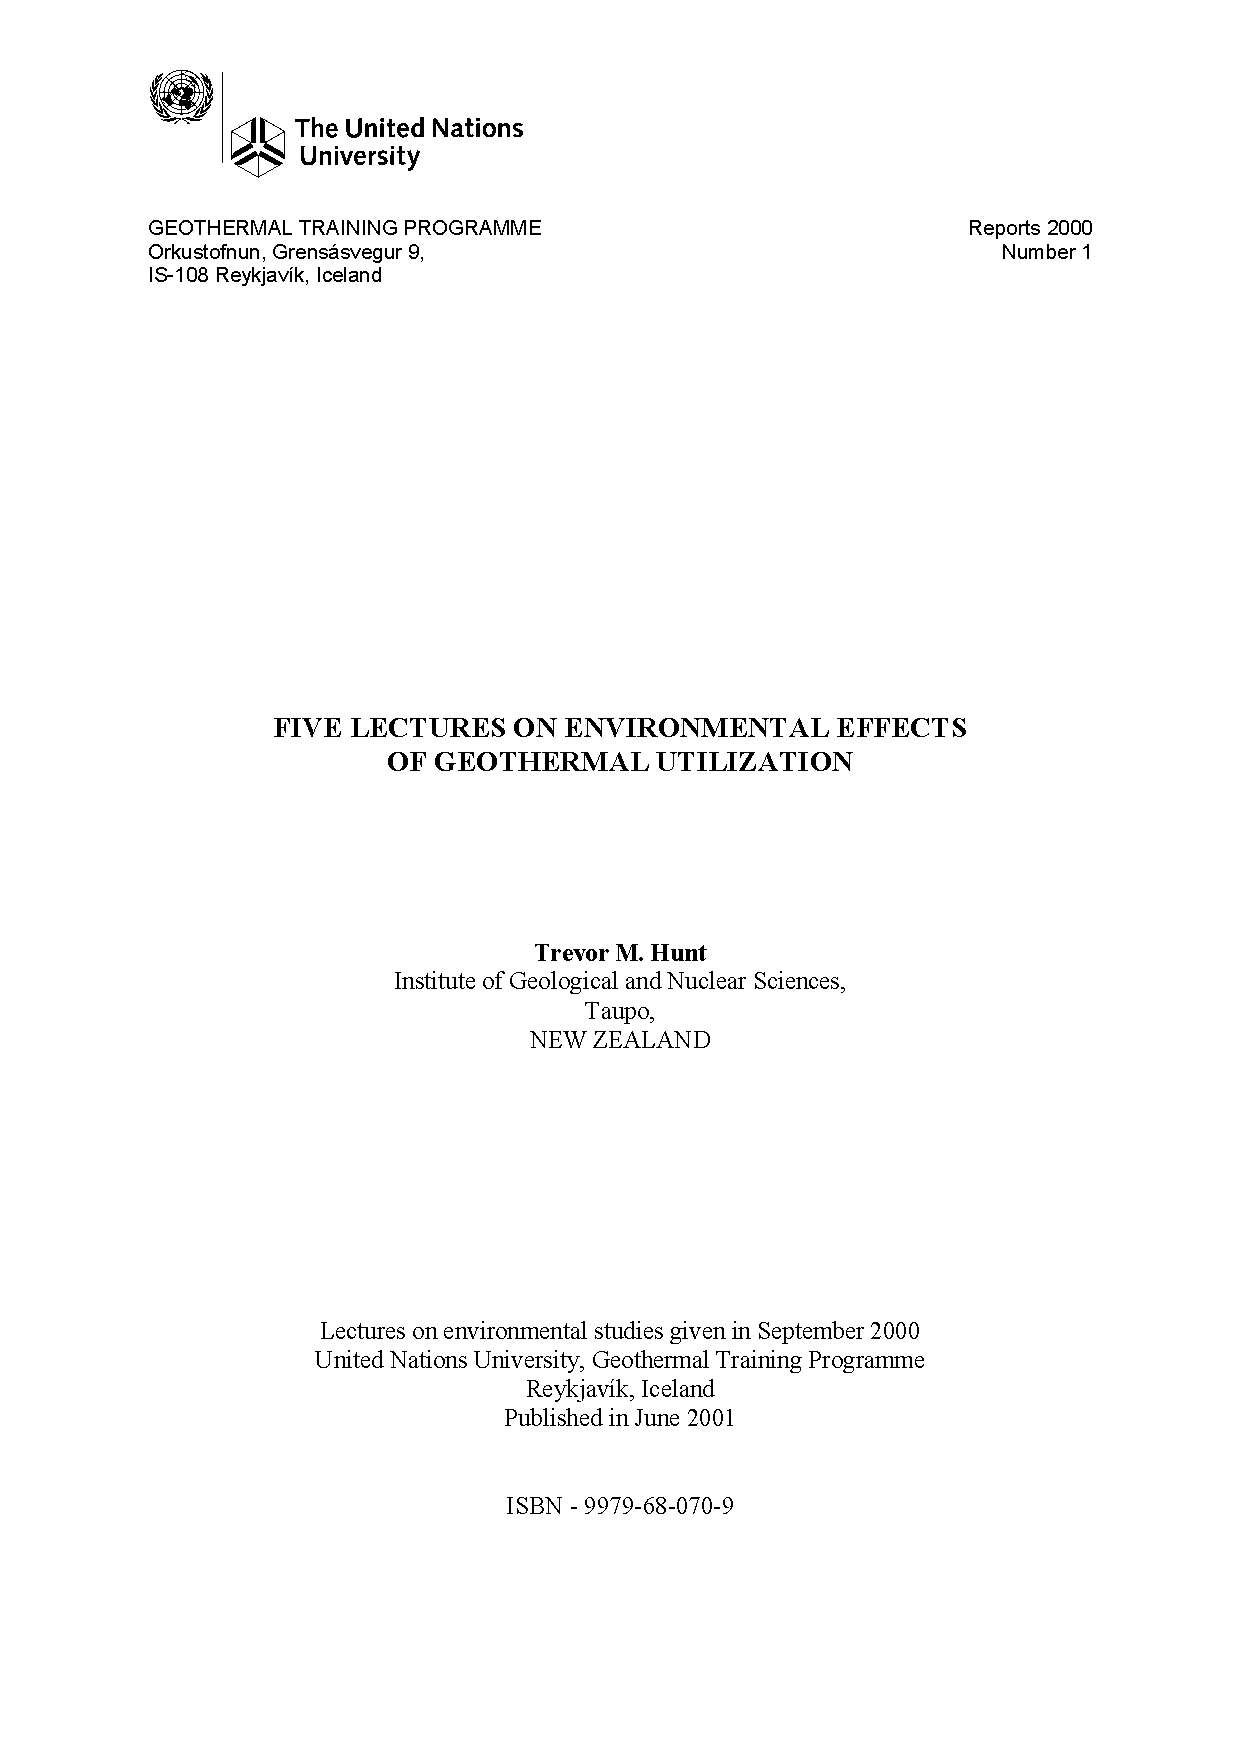
\includepdf[pages=-,fitpaper, angle=0]{./HuntSelect.pdf}
%}

\end{document}
